\documentclass[a4paper, 12pt]{article}
\usepackage[utf8x]{inputenc}
\usepackage{cmap}
\usepackage[english, russian]{babel}
\usepackage{indentfirst}
\usepackage[left=20mm, top=20mm, right=20mm, bottom=20mm]{geometry}
\usepackage{tikz}
\usepackage{float}
\usepackage{amsmath, amsfonts, amssymb}
\usepackage{graphicx}
\usepackage{fancybox, fancyhdr}
\usepackage{hyperref}
\usepackage{listings}
\usepackage{caption}
\usepackage{subcaption}
\usepackage{xcolor}
\usepackage{paralist}
\usepackage{tabularx}
\pagestyle{fancy}
\fancyhf{}
\fancyhead[L]{Лабораторная работа №4}
\fancyhead[R]{Программирование промышленных роботов}
\fancyfoot[C]{\thepage}
\graphicspath{{images/}}
\usetikzlibrary{patterns}
\definecolor{LightGray}{gray}{0.95}
\definecolor{LightGray2}{gray}{0.7}
\lstdefinelanguage{MELFABASIC}{
    keywords={MVS, MVR, JOVRD,
              HOPEN, HCLOSE, DLY,
              MOV, END, OPEN,
              CLOSE, FOR,, TO,
              NEXT},
    sensitive=true,
    comment=[*],
    morecomment=[l]{;},
    morestring=[b]"
}
\lstdefinestyle{code}{
    language=MELFABASIC, % replace with needed language
    basicstyle=\footnotesize\ttfamily,
    backgroundcolor=\color{LightGray},
    showspaces=false,
    showstringspaces=false,
    showtabs=false,
    tabsize=4,
    captionpos=b,
    breaklines=true,
    breakatwhitespace=false,
    frame=single,
    rulecolor=\color{LightGray2},
    linewidth=\linewidth,
    keywordstyle=\color{blue}\bfseries,
    commentstyle=\color{green!40!black},
    stringstyle=\color{red},
    escapeinside={\%*}{*)},
    inputencoding=utf8x,
    xleftmargin=0pt,
    framexleftmargin=0pt,
    framexrightmargin=0pt
}
\lstdefinestyle{python}{
    language=python, % replace with needed language
    basicstyle=\footnotesize\ttfamily,
    backgroundcolor=\color{LightGray},
    showspaces=false,
    showstringspaces=false,
    showtabs=false,
    tabsize=4,
    captionpos=b,
    breaklines=true,
    breakatwhitespace=false,
    frame=single,
    rulecolor=\color{LightGray2},
    linewidth=\linewidth,
    keywordstyle=\color{blue}\bfseries,
    commentstyle=\color{green!40!black},
    stringstyle=\color{red},
    escapeinside={\%*}{*)},
    inputencoding=utf8x,
    xleftmargin=0pt,
    framexleftmargin=0pt,
    framexrightmargin=0pt
}
\lstset{style=code}
\hypersetup{
    colorlinks=true,
    linkcolor=blue,
    filecolor=magenta,
    urlcolor=cyan,
    pdftitle={contents setup},
    pdfpagemode=FullScreen,
}
\setlength{\parskip}{1.5mm}
\setlength{\headheight}{15pt}
\setlength{\footskip}{15pt}
\allowdisplaybreaks
\DeclareMathOperator{\sinc}{sinc}
\newcommand{\frc}[2]{\raisebox{2pt}{$#1$}\big/\raisebox{-3pt}{$#2$}}

\begin{document}
    \begin{titlepage}

        \begin{center}
        
\includegraphics[width=0.3\textwidth]{itmo.png} % requires itmo.png in /images folder
        \vfill
        
        Федеральное государственное автономное образовательное учреждение высшего образования
        «Национальный Исследовательский Университет ИТМО»\\
        
        \vfill
        {\large\bf ЛАБОРАТОРНАЯ РАБОТА №4}\\
        {\large\bf «ПРОГРАММИРОВАНИЕ ПРОМЫШЛЕННЫХ РОБОТОВ»}\\
        {\large\bf «СЕТЕВЫЕ СООБЩЕНИЯ»}
        \vfill

        \begin{flushright}
            \begin{minipage}{.45\textwidth}
            {
                \hbox{Преподаватель:}
                \hbox{Громов В. С.}
                \hbox{}
                \hbox{Выполнили:}
                \hbox{Румянцев А. А., R3341}
                \hbox{Чебаненко Д. А., R3341}
                \hbox{Овчинников П. А., R3341}
                \hbox{Блохин С. О., R3342}
                \hbox{Тоскано О. Арасели Д. П., R3338}
                \hbox{}
                \hbox{Факультет: СУиР}
            }
            \end{minipage}
        \end{flushright}
        
        \vfill
                
        Санкт-Петербург\\
        2024
        \end{center}
    \end{titlepage}
    
    \tableofcontents

    \newpage
    \section{Цели выполнения работы}
    Написать программу, которая будет считывать из TCP/IP порта 10003
    номера деталей по осям X и Y (от 0 до 2 по каждой из осей), затем
    переносить указанную деталь с первого стола с деталями на второй
    пустой стол. На втором столе детали следует выкладывать
    последовательно линиями. Указанные операции должны производиться
    9 раз (по общему числу деталей).


    \section{Код конечной программы}
    \subsection{MELFA BASIC}
    \begin{figure}[H]
        \centering
        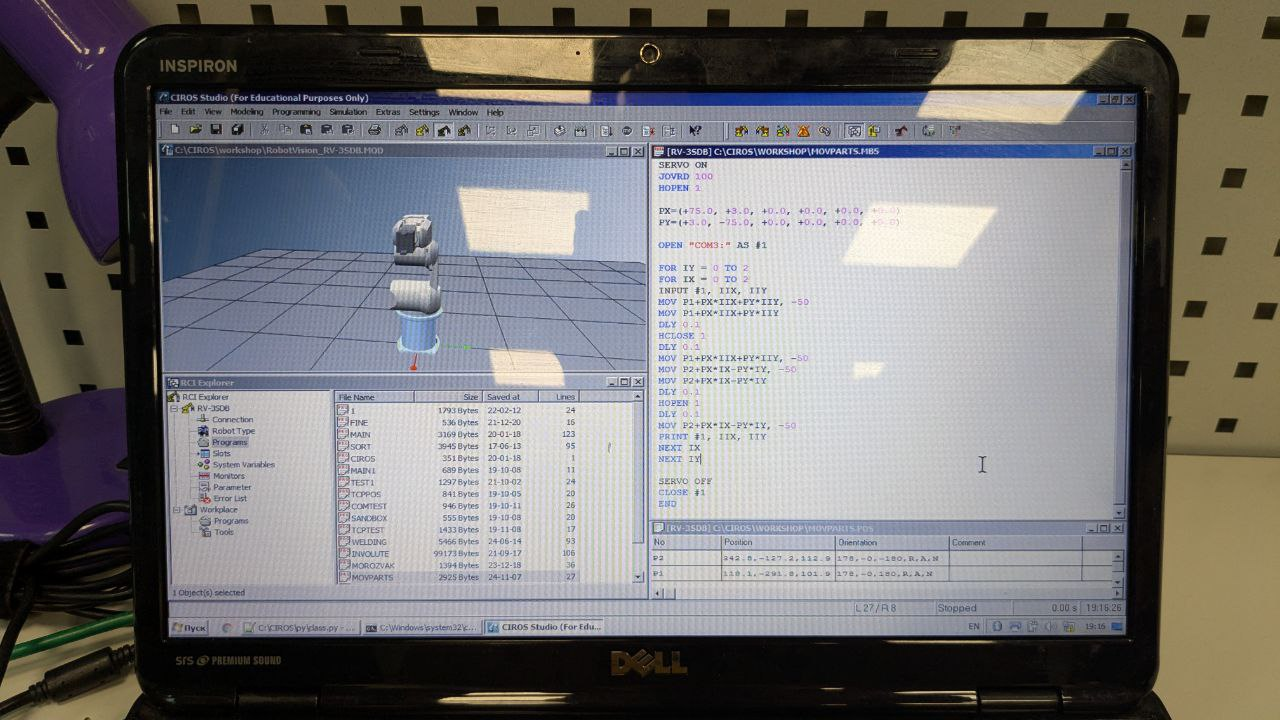
\includegraphics[scale=0.36]{code.jpg}
        \captionsetup{skip=0pt}
        \caption{Фото конечной программы на языке \texttt{MELFA BASIC}}
        \label{fig:codephoto}
    \end{figure}
    \begin{lstlisting}[label=code, caption={Листинг конечной программы на языке \texttt{MELFA BASIC}}]
    SERVO ON
    JOVRD 100
    HOPEN 1

    PX=(+75.0, +3.0, +0.0, +0.0, +0.0, +0.0)
    PY=(+3.0, -75.0, +0.0, +0.0, +0.0, +0.0)

    OPEN "COM3:" AS #1

    FOR IY = 0 TO 2
    FOR IX = 0 TO 2
    INPUT #1, IIX, IIY
    MOV P1+PX*IIX+PY*IIY, -50
    MOV P1+PX*IIX+PY*IIY
    DLY 0.1
    HCLOSE 1
    DLY 0.1
    MOV P1+PX*IIX+PY*IIY, -50
    MOV P2+PX*IX-PY*IY, -50
    MOV P2+PX*IX-PY*IY
    DLY 0.1
    HOPEN 1
    DLY 0.1
    MOV P2+PX*IX-PY*IY, -50
    PRINT #1, IIX, IIY
    NEXT IX
    NEXT IY

    SERVO OFF
    CLOSE #1
    END
    \end{lstlisting}


    \subsection{Python}
    \begin{figure}[H]
        \centering
        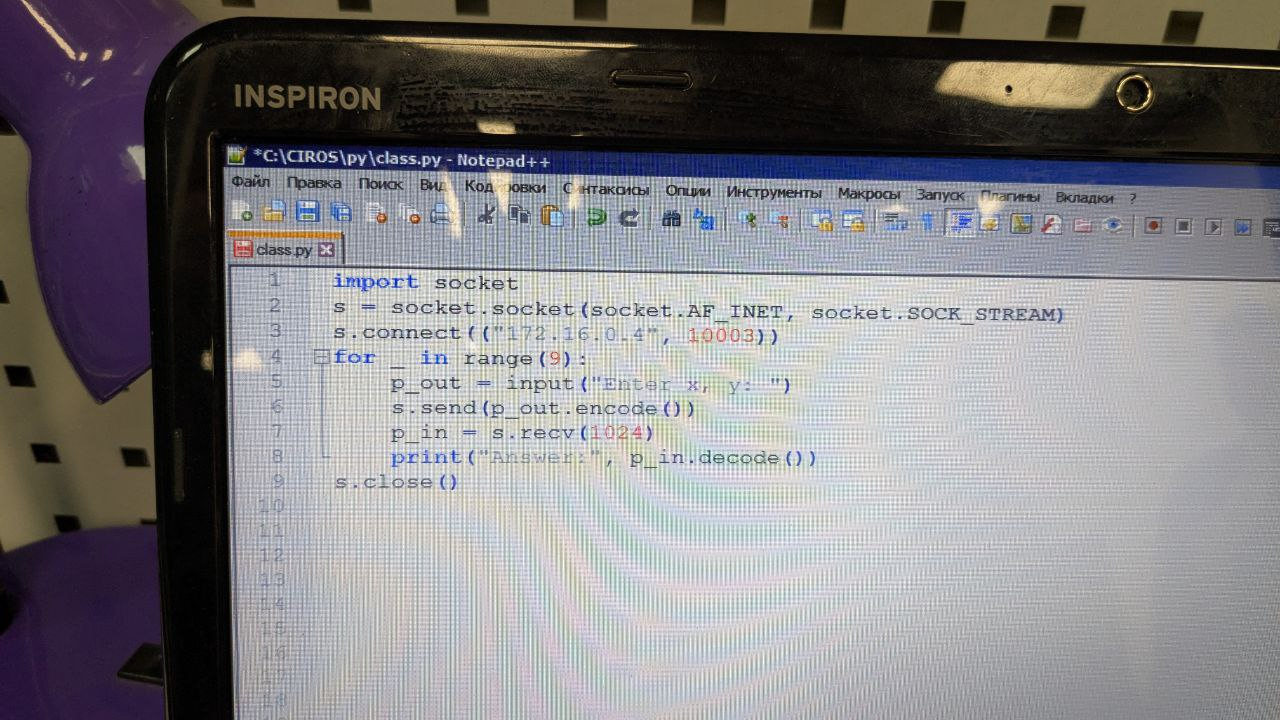
\includegraphics[scale=0.36]{code2.jpg}
        \captionsetup{skip=0pt}
        \caption{Фото конечной программы на языке \texttt{Python}}
        \label{fig:codephoto2}
    \end{figure}
    \begin{lstlisting}[style=python, label=code2, caption={Листинг конечной программы на языке \texttt{Python}}]
    import socket
    s = socket.socket(socket.AF_INET, socket.SOCK_STREAM)
    s.connect(("172.16.0.4", 10003))
    for _ in range(9):
        p_out = input("Enter x, y: ")
        s.send(p_out.encode())
        p_in = s.recv(1024)
        print("Answer:", p_in.decode())
    s.close()
    \end{lstlisting}


    \subsection{Описание команд}
    При выполнении лабораторной работы использовались следующие команды программирования языка \texttt{MELFA BASIC}:
    \begin{compactitem}
    \item \texttt{END} -- завершение программы
    \item \texttt{SERVO ON} -- включение двигателей
    \item \texttt{JOVRD 100} -- скорость движения в процентах от максимальной
    \item \texttt{SERVO OFF} -- выключение двигателей
    \item \texttt{DLY 0.1} -- пауза выполнения программы в секундах
    \item \texttt{HOPEN 1} -- открытие захватного устройства
    \item \texttt{HCLOSE 1} -- закрытие захватного устройства 
    \item \texttt{PX=(+75.0, +3.0, +0.0, +0.0, +0.0, +0.0)} -- вспомогательная переменная координат формата (X, Y, Z, A, B, C) с декартовыми координатами для создания настраиваемого смещения координат
    \item \texttt{OPEN "COM3:" AS \#1} -- открытие TCP/IP порта 10003 для подключения интерфейса \#1
    \item \texttt{CLOSE \#1} -- закрытие TCP/IP порта 10003 для подключения интерфейса \#1
    \item \texttt{FOR IY = 0 TO 2} -- начало выполнения цикла, IY -- переменная итерации цикла
    \item \texttt{NEXT IY} -- окончание цикла
    \item \texttt{INPUT \#1, IIX, IIY} -- считывание содержимого буфера интерфейса \#1 в переменные IIX и IIY
    \item \texttt{PRINT \#1, IIX, IIY} -- вывод содержимого переменных IIX и IIY в интерфейс \#1
    \item \texttt{MOV P1+PX*IIX+PY*IIY} -- движение в точку P1 из таблицы сохраненных точек с положительным смещением PX*IIX+PY*IIY
    \item \texttt{MOV P1+PX*IIX+PY*IIY, -50} -- движение в точку P1 из таблицы сохраненных точек с положительным смещением PX*IIX+PY*IIY и 50 мм вверх по оси Z
    \end{compactitem}
    А также следующие команды программирования языка \texttt{Python}:
    \begin{compactitem}
        \item \texttt{import socket} -- импорт модуля для работы с сетевыми соединениями
        \item \texttt{s = socket.socket(...)} -- создаем TCP-сокет для соединения с роботом
        \item \texttt{s.connect(...)} -- подключаемся к роботу по IP адресу и порту
        \item \texttt{for \_ in range(9)} -- цикл с количеством итераций равным количеству деталей
        \item \texttt{p\_out = input(...)} -- запрос у пользователя ввода координат
        \item \texttt{s.send(p\_out.encode())} -- отправка роботу строки в виде байтового формата
        \item \texttt{p\_in = s.recv(1024)} -- получение ответа от робота (макс. размер данных 1024 байта)
        \item \texttt{print(...)} -- вывод ответа робота в консоль
        \item \texttt{s.close()} -- закрытие соединения с роботом
    \end{compactitem}


    \section{Таблица сохраненных точек}
    \begin{figure}[H]
        \centering
        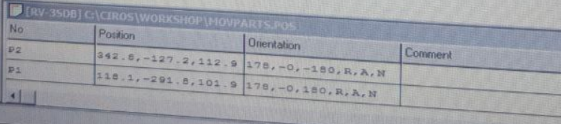
\includegraphics[scale=1.35]{table.png}
        \captionsetup{skip=0pt}
        \caption{Фото таблицы с сохраненными точками}
        \label{fig:table}
    \end{figure}
    \begin{tabularx}{0.92\textwidth} { 
        | >{\raggedright\arraybackslash}X 
        | >{\raggedright\arraybackslash}X 
        | >{\raggedright\arraybackslash}X | }
       \hline
       No & Position & Orientation \\
       \hline
       P1 & $118.1, -291.8, 101.9$ & $178, -0, 180$, R, A, N \\
       \hline
       P2 & $342.6, -127.2, 112.9$ & $178, -0, -180$, R, A, N \\
      \hline
    \end{tabularx}


    \section{Этапы выполнения программы}
    \begin{figure}[H]
        \centering
        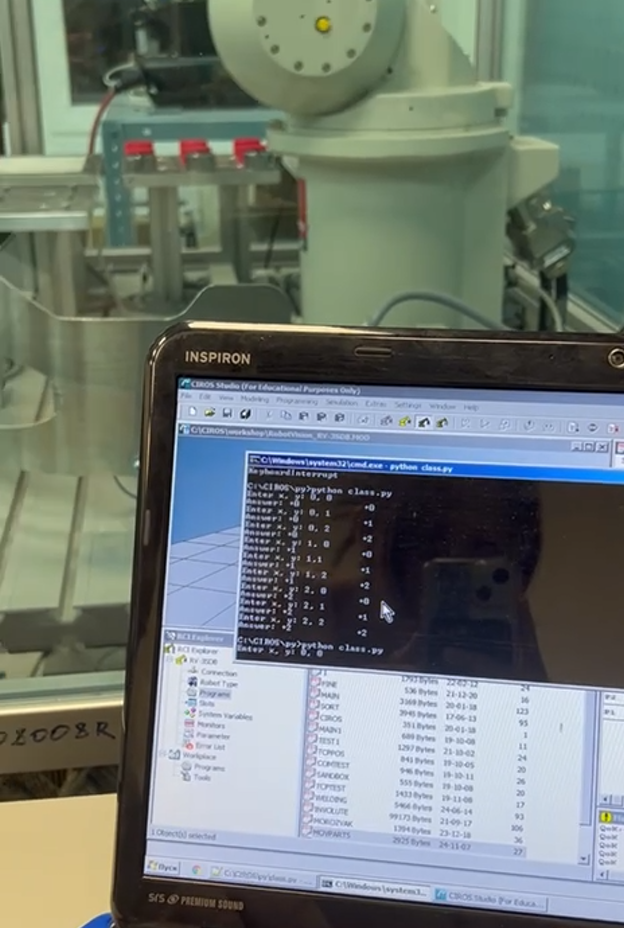
\includegraphics[scale=1]{input00.png}
        \captionsetup{skip=0pt}
        \caption{Ввод координаты точки (0, 0) в консоль с запущенным \texttt{Python} скриптом}
        \label{fig:input00}
    \end{figure}
    \begin{figure}[H]
        \centering
        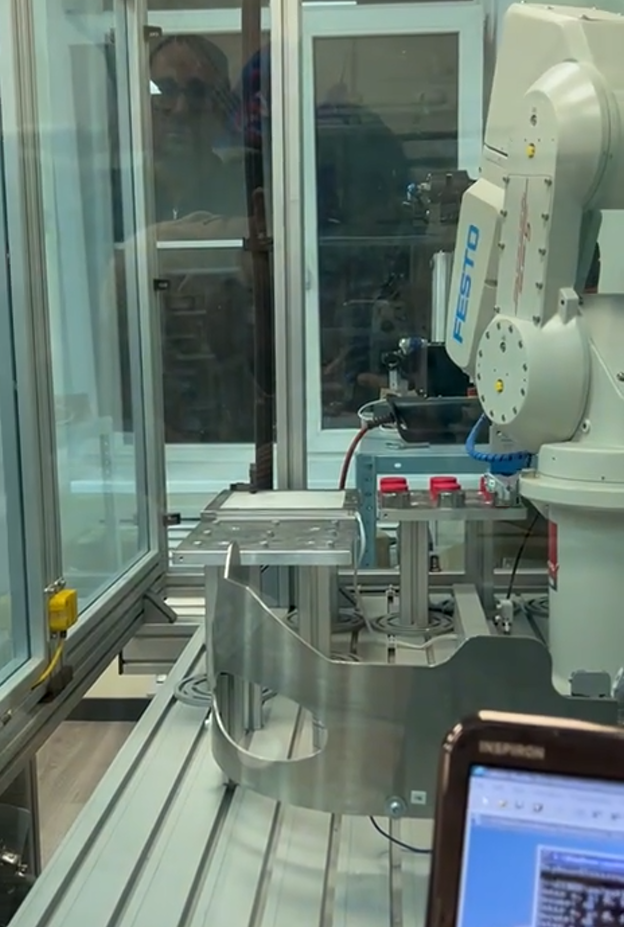
\includegraphics[scale=1]{take00.png}
        \captionsetup{skip=0pt}
        \caption{Робот берет деталь с позиции (0, 0)}
        \label{fig:take00}
    \end{figure}
    \begin{figure}[H]
        \centering
        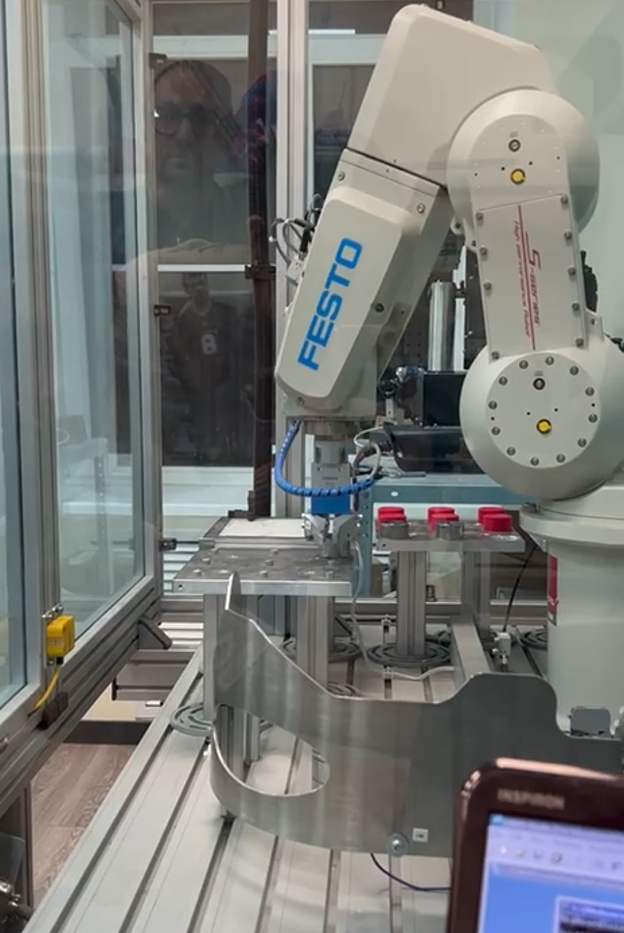
\includegraphics[scale=1]{put00.png}
        \captionsetup{skip=0pt}
        \caption{Робот кладет деталь в начальную для последовательного переноса точку}
        \label{fig:put00}
    \end{figure}
    \begin{figure}[H]
        \centering
        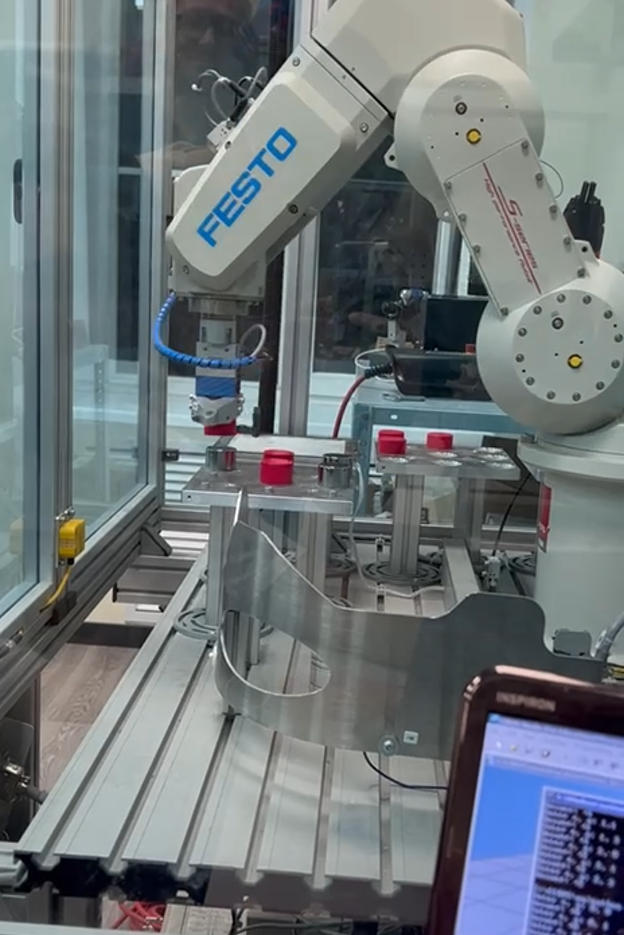
\includegraphics[scale=1]{repeat.png}
        \captionsetup{skip=0pt}
        \caption{Робот продолжает переносить детали с задаваемых координат с первого стола на второй, размещая их последовательно}
        \label{fig:repeat}
    \end{figure}


    \newpage
    \section{Выводы}
    В результате выполнения лабораторной работы мы:
    \begin{compactitem}
        \item познакомились с передачей TCP/IP пакетов с компьютера на робот и обратно
        \item написали программу на языке \texttt{MELFA BASIC} для размещения
        роботом деталей на второй стол в последовательном порядке в соответствии
        с вводимыми в консоль с запущенным скриптом на языке \texttt{Python}
        координатами деталей с первого стола
    \end{compactitem}
\end{document}